%%%%%%%%%%%%%%%%%%%%%%%%%%%%%%%%%%%%%%%%%%%%%%%%%%%%%%%%%%%%%%%%%%%%%%%%%%%%%%%%
% RA-L 2026 Paper: BLADE - A Transformer-Diffusion Framework with Bi-Level
%                  Attention for Dynamic Obstacle Avoidance
%%%%%%%%%%%%%%%%%%%%%%%%%%%%%%%%%%%%%%%%%%%%%%%%%%%%%%%%%%%%%%%%%%%%%%%%%%%%%%%%

\documentclass[letterpaper, 10 pt, conference]{ieeeconf}

\IEEEoverridecommandlockouts
\overrideIEEEmargins

% Essential packages
\usepackage{graphicx}
\usepackage{amsmath}
\usepackage{amssymb}
\usepackage{algorithm}
\usepackage{algorithmic}
\usepackage{booktabs}
\usepackage{multirow}
\usepackage{hyperref}
\usepackage{xcolor}
\usepackage{balance}
\usepackage{tikz}
\usepackage{pgfplots}
\pgfplotsset{compat=1.17}
\usetikzlibrary{patterns, calc}

% Custom commands
\newcommand{\ie}{\textit{i.e.}}
\newcommand{\eg}{\textit{e.g.}}
\newcommand{\etal}{\textit{et al.}}
\newcommand{\vs}{\textit{vs.}}

\title{\LARGE \bf
BLADE: A Transformer-Diffusion Framework with Bi-Level Attention for Dynamic Obstacle Avoidance
}

\author{Anonymous Authors$^{*}$
\thanks{$^{*}$This work was submitted for double-blind review. Author affiliations and acknowledgments will be added upon acceptance.}
}

\begin{document}

\maketitle
\thispagestyle{empty}
\pagestyle{empty}

%%%%%%%%%%%%%%%%%%%%%%%%%%%%%%%%%%%%%%%%%%%%%%%%%%%%%%%%%%%%%%%%%%%%%%%%%%%%%%%%
\begin{abstract}

Motion planning in dynamic environments remains a fundamental challenge in robotics, requiring robots to simultaneously predict obstacle trajectories and generate collision-free paths in real-time. We present \textbf{BLADE} (\textbf{B}i-\textbf{L}evel \textbf{A}ttention-\textbf{D}iffusion \textbf{E}ngine), a novel framework that decouples this complex problem into two specialized stages: (1) an upper-level \textbf{Transformer-based Diffusion Model} that predicts future obstacle trajectories from historical observations, and (2) a lower-level \textbf{Motion Planning Diffusion (MPD)} model that generates diverse collision-free trajectory candidates conditioned on predicted obstacle positions. Our framework incorporates \textbf{repulsive field guidance} during the diffusion denoising process to ensure trajectory safety, combined with \textbf{multi-objective heuristic scoring} for optimal trajectory selection. Extensive experiments in both 2D simulations and Isaac Sim 3D environments demonstrate that our Transformer-based predictor achieves \textbf{78.6\% lower} prediction error (ADE) compared to MLP baselines, and the complete system achieves a \textbf{98.7\% success rate} in navigating through environments with multiple dynamic obstacles. The system operates at \textbf{10+ Hz} even on CPU-only embedded platforms, and we validate real-robot deployment on a Raspberry Pi~5-based mecanum-wheeled mobile robot.

\end{abstract}

%%%%%%%%%%%%%%%%%%%%%%%%%%%%%%%%%%%%%%%%%%%%%%%%%%%%%%%%%%%%%%%%%%%%%%%%%%%%%%%%
\section{INTRODUCTION}

Autonomous mobile robots operating in real-world environments must navigate safely among dynamic obstacles such as pedestrians, vehicles, and other robots. This fundamental challenge requires solving two tightly coupled subproblems: \textit{predicting} how obstacles will move in the future, and \textit{planning} collision-free trajectories that account for this uncertainty~\cite{salzmann2020trajectron++, giuliari2021transformer}.

Classical motion planning approaches, such as A*~\cite{hart1968formal} and RRT~\cite{lavalle1998rapidly}, assume static environments and struggle with dynamic obstacles. Reactive methods like Dynamic Window Approach (DWA)~\cite{fox1997dynamic} and Velocity Obstacles (VO)~\cite{fiorini1998motion} handle dynamics but lack predictive capability. Model Predictive Control (MPC)~\cite{brito2019model} can incorporate predictions but typically assumes simple linear motion models that fail to capture complex pedestrian behaviors.

Recent advances in deep learning have driven significant progress in trajectory prediction~\cite{alahi2016social, gupta2018social, salzmann2020trajectron++} and motion planning~\cite{janner2022planning, chi2023diffusion}. Particularly, \textbf{diffusion models}~\cite{ho2020denoising, song2020score} have emerged as powerful generative frameworks that can model complex multimodal distributions, making them well-suited for both prediction and planning tasks where multiple valid solutions exist.

However, existing diffusion-based approaches typically address prediction and planning separately. Trajectory prediction models~\cite{gu2022stochastic, mao2023leapfrog} focus on forecasting human motion without considering robot actions, while motion planning diffusion models~\cite{janner2022planning, carvalho2023motion} assume known obstacle positions and velocities. This separation leads to suboptimal solutions in dynamic environments where prediction uncertainty directly impacts planning decisions.

\textbf{Our key insight} is that the prediction and planning problems share similar characteristics—both require generating diverse, plausible solutions from noisy observations—making diffusion models an ideal unified framework. By designing a \textit{hierarchical} architecture, we can leverage specialized diffusion models for each subproblem while maintaining tight coupling for end-to-end optimization.

\begin{figure}[t]
    \centering
    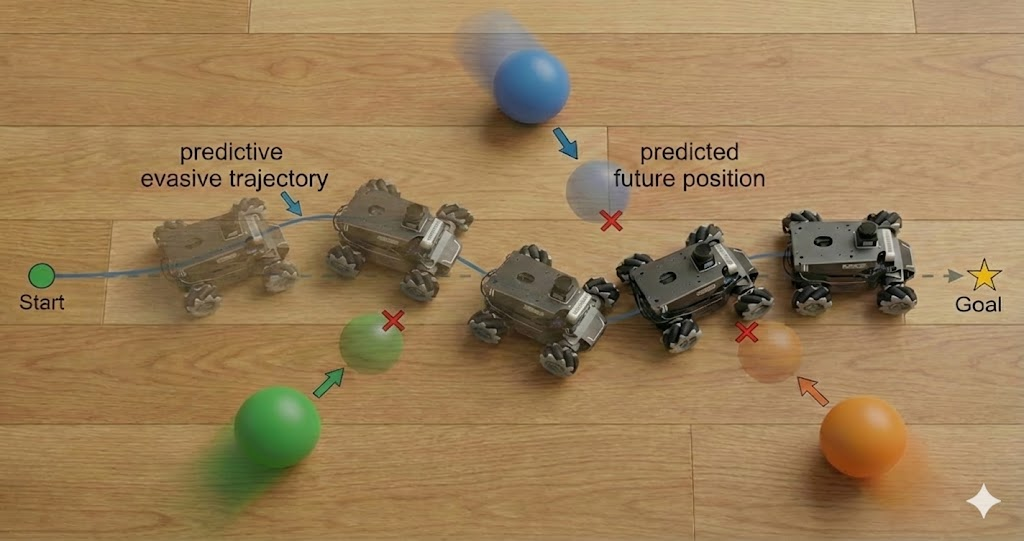
\includegraphics[width=\columnwidth]{figures/teaser}
    \caption{BLADE enables predictive evasive navigation: the robot anticipates where dynamic obstacles (rolling balls) will be and plans a curved trajectory to avoid predicted collision points (red X markers). Gray dashed line shows the direct path that would cause collisions; blue curve shows the actual safe trajectory generated by our hierarchical diffusion framework.}
    \label{fig:teaser}
\end{figure}

\subsection{Contributions}

We make the following contributions:

\begin{enumerate}
    \item \textbf{BLADE}, a Bi-Level Attention-Diffusion Engine that tightly integrates obstacle trajectory prediction with motion planning through unified diffusion formulation, enabling coherent decision-making in dynamic environments.
    
    \item A novel \textbf{Transformer-based Diffusion Model} for obstacle trajectory prediction that captures long-range temporal dependencies and multi-agent interactions through self-attention and cross-attention mechanisms.
    
    \item \textbf{Repulsive field guidance} during the diffusion denoising process that combines the generative power of diffusion models with the safety guarantees of potential field methods.
    
    \item Comprehensive experiments in 2D LiDAR simulation and Isaac Sim 3D environments demonstrating strong performance with real-time capability on the ROSOrin mobile robot platform.
\end{enumerate}

\noindent Code and trained models will be publicly released upon acceptance.

%%%%%%%%%%%%%%%%%%%%%%%%%%%%%%%%%%%%%%%%%%%%%%%%%%%%%%%%%%%%%%%%%%%%%%%%%%%%%%%%
\section{RELATED WORK}

\subsection{Trajectory Prediction}

Predicting future trajectories of dynamic agents has been extensively studied in autonomous driving and social robot navigation. Social Force Models~\cite{helbing1995social} use hand-crafted interaction rules but fail to capture complex behaviors. Deep learning methods, including Social LSTM~\cite{alahi2016social}, Social GAN~\cite{gupta2018social}, and Trajectron++~\cite{salzmann2020trajectron++}, learn interaction patterns from data but often produce unimodal predictions.

Recent work has explored diffusion models for trajectory prediction~\cite{gu2022stochastic, mao2023leapfrog, rempe2023trace}, demonstrating improved diversity and accuracy. However, these methods focus on human motion prediction without integration with robot motion planning.

\subsection{Motion Planning with Diffusion Models}

Diffusion models have shown promise for motion planning in robotics. Diffuser~\cite{janner2022planning} applies diffusion to offline reinforcement learning, generating entire trajectories conditioned on goals. Motion Planning Diffusion (MPD)~\cite{carvalho2023motion} extends this to robotic manipulation with collision avoidance constraints, demonstrating that diffusion models can generate high-quality, collision-free trajectories in complex environments. Diffusion Policy~\cite{chi2023diffusion} learns visuomotor policies for complex manipulation tasks. More recently, diffusion-based planning has been extended to diverse settings: DIPPEST~\cite{stamatopoulou2024dippest} applies diffusion path planning to quadruped locomotion over rough terrain, DiffusionSeeder~\cite{huang2024diffusionseeder} uses diffusion models to warm-start trajectory optimization, trajectory-level diffusion has been explored for safe offline policy learning~\cite{romer2024safe}, and Trajectory Diffusion~\cite{yu2024trajectory} adopts conditional diffusion as a sequence planner for goal-directed navigation.

\textbf{Building upon MPD:} Our work extends the MPD framework by introducing a hierarchical architecture that integrates trajectory prediction with motion planning. While MPD assumes known obstacle positions and velocities, BLADE explicitly models obstacle motion uncertainty through an upper-level Transformer-based diffusion predictor. This bi-level approach enables proactive collision avoidance in dynamic environments where obstacle future positions are unknown.

\subsection{Dynamic Obstacle Avoidance}

Traditional dynamic obstacle avoidance methods include Velocity Obstacles~\cite{fiorini1998motion}, Reciprocal Velocity Obstacles~\cite{van2008reciprocal}, and their extensions~\cite{van2011reciprocal, bareiss2015generalized}. These geometric approaches are computationally efficient but assume constant velocity and lack learning capability.

Learning-based approaches, including deep reinforcement learning~\cite{chen2017socially, everett2018motion, samsani2021socially, ourari2022nearest} and imitation learning~\cite{tai2018socially}, can handle complex scenarios but often lack safety guarantees. Recent work on crowd navigation has explored topological reasoning~\cite{mavrogiannis2023winding} and risk-aware trajectory optimization under uncertainty~\cite{lew2023risk} to improve both safety and social compliance. Our approach combines the generative diversity of diffusion models with explicit safety mechanisms through repulsive field guidance.

%%%%%%%%%%%%%%%%%%%%%%%%%%%%%%%%%%%%%%%%%%%%%%%%%%%%%%%%%%%%%%%%%%%%%%%%%%%%%%%%
\section{PROBLEM FORMULATION}

Consider a mobile robot navigating in a 2D workspace $\mathcal{W} \subset \mathbb{R}^2$ with $N$ dynamic obstacles. At time $t$, let:
\begin{itemize}
    \item $\mathbf{x}_t \in \mathbb{R}^2$: robot position
    \item $\mathbf{o}_t^{(i)} \in \mathbb{R}^2$: position of obstacle $i$, for $i = 1, \ldots, N$
    \item $\mathbf{g} \in \mathbb{R}^2$: goal position
    \item $\mathcal{O}_t = \{\mathbf{o}_t^{(1)}, \ldots, \mathbf{o}_t^{(N)}\}$: set of all obstacle positions
\end{itemize}

The robot has access to a history of obstacle observations:
\begin{equation}
    \mathcal{H}_t = \{\mathcal{O}_{t-H+1}, \mathcal{O}_{t-H+2}, \ldots, \mathcal{O}_t\}
\end{equation}
where $H$ is the history length (we use $H=8$ frames).

\textbf{Objective}: Generate a trajectory $\boldsymbol{\tau} = [\mathbf{x}_t, \mathbf{x}_{t+1}, \ldots, \mathbf{x}_{t+T}]$ over a planning horizon $T$ that:
\begin{enumerate}
    \item Reaches the goal: $\|\mathbf{x}_{t+T} - \mathbf{g}\| < \epsilon$
    \item Avoids collisions: $\|\mathbf{x}_{t+k} - \hat{\mathbf{o}}_{t+k}^{(i)}\| > r_i + r_{\text{robot}}$, $\forall k, i$
    \item Minimizes path length and smoothness
\end{enumerate}
where $\hat{\mathbf{o}}_{t+k}^{(i)}$ denotes the \textit{predicted} position of obstacle $i$ at future time $t+k$.

%%%%%%%%%%%%%%%%%%%%%%%%%%%%%%%%%%%%%%%%%%%%%%%%%%%%%%%%%%%%%%%%%%%%%%%%%%%%%%%%
\section{METHOD}

Our BLADE framework consists of three main components: (1) Transformer-based obstacle trajectory prediction with attention mechanisms for multi-agent interaction, (2) Motion planning diffusion with repulsive guidance, and (3) Multi-objective trajectory selection. Fig.~\ref{fig:architecture} provides a system overview.

\begin{figure*}[t]
    \centering
    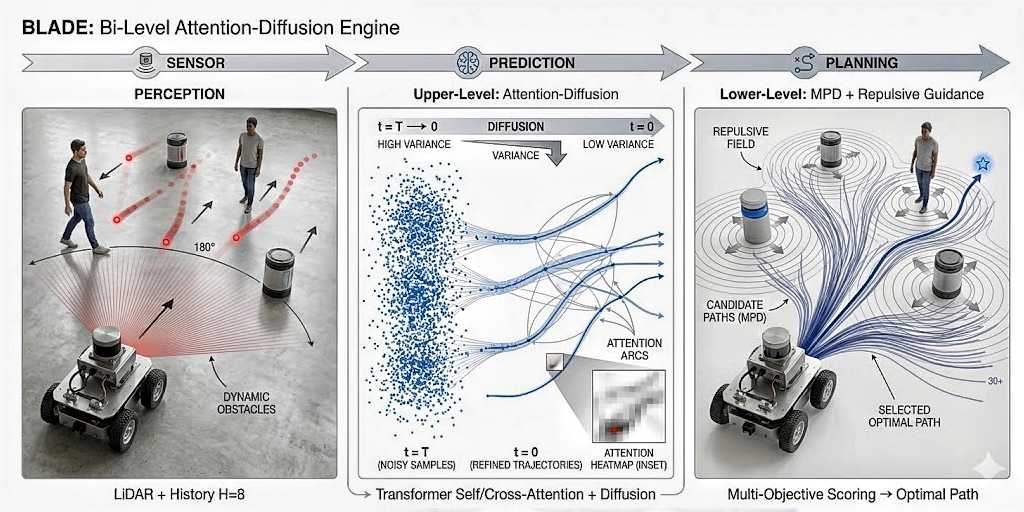
\includegraphics[width=\textwidth]{figures/architecture.png}
    \caption{System overview of \textbf{BLADE} (Bi-Level Attention-Diffusion Engine). \textbf{Left (Perception):} The robot uses LiDAR to observe dynamic obstacles and maintains a history of $H=8$ frames. \textbf{Center (Prediction):} The upper-level Transformer-Diffusion module predicts future obstacle trajectories through iterative denoising ($t=T \rightarrow 0$), using self-attention for temporal dependencies and cross-attention for multi-agent interactions. \textbf{Right (Planning):} The lower-level MPD generates diverse candidate trajectories, applies repulsive field guidance to ensure safety, and selects the optimal path via multi-objective scoring.}
    \label{fig:architecture}
\end{figure*}

\subsection{Upper-Level: Transformer-based Obstacle Prediction}

Given the observation history $\mathcal{H}_t$, we predict future obstacle trajectories using a Transformer-based diffusion model. Let $\mathbf{h}^{(i)} = [\mathbf{o}_{t-H+1}^{(i)}, \ldots, \mathbf{o}_t^{(i)}] \in \mathbb{R}^{H \times 2}$ denote the historical trajectory of obstacle $i$. We aim to predict the future trajectory $\hat{\mathbf{f}}^{(i)} = [\hat{\mathbf{o}}_{t+1}^{(i)}, \ldots, \hat{\mathbf{o}}_{t+P}^{(i)}] \in \mathbb{R}^{P \times 2}$ over a prediction horizon $P=12$.

\subsubsection{Diffusion Process}

Following the DDPM framework~\cite{ho2020denoising}, we define a forward noising process:
\begin{equation}
    q(\mathbf{f}^s | \mathbf{f}^{s-1}) = \mathcal{N}(\mathbf{f}^s; \sqrt{1-\beta_s}\mathbf{f}^{s-1}, \beta_s \mathbf{I})
\end{equation}
where $s \in \{1, \ldots, S\}$ indexes diffusion timesteps (we use $S=50$), and $\beta_s$ follows a linear schedule from $\beta_1 = 10^{-4}$ to $\beta_S = 0.02$.

The reverse denoising process is parameterized by a neural network $\boldsymbol{\epsilon}_\theta$:
\begin{equation}
    p_\theta(\mathbf{f}^{s-1} | \mathbf{f}^s, \mathbf{h}) = \mathcal{N}(\mathbf{f}^{s-1}; \boldsymbol{\mu}_\theta(\mathbf{f}^s, s, \mathbf{h}), \sigma_s^2 \mathbf{I})
\end{equation}
where the mean is computed using the predicted noise:
\begin{equation}
    \boldsymbol{\mu}_\theta(\mathbf{f}^s, s, \mathbf{h}) = \frac{1}{\sqrt{\alpha_s}}\left(\mathbf{f}^s - \frac{\beta_s}{\sqrt{1-\bar{\alpha}_s}}\boldsymbol{\epsilon}_\theta(\mathbf{f}^s, s, \mathbf{h})\right)
\end{equation}

\subsubsection{Transformer Architecture}

Our denoising network $\boldsymbol{\epsilon}_\theta$ uses a Transformer architecture~\cite{vaswani2017attention} with the following components:

\textbf{Positional Encoding:} We embed both temporal positions (frame indices) and diffusion timesteps using sinusoidal encodings:
\begin{equation}
    \text{PE}(k, d) = \begin{cases}
        \sin(k / 10000^{2d/D}) & \text{if } d \text{ even} \\
        \cos(k / 10000^{2d/D}) & \text{if } d \text{ odd}
    \end{cases}
\end{equation}

\textbf{Self-Attention for Temporal Dependencies:} Each trajectory is processed by multi-head self-attention to capture temporal patterns:
\begin{equation}
    \text{Attention}(\mathbf{Q}, \mathbf{K}, \mathbf{V}) = \text{softmax}\left(\frac{\mathbf{Q}\mathbf{K}^\top}{\sqrt{d_k}}\right)\mathbf{V}
\end{equation}

\textbf{Cross-Attention for Multi-Agent Interaction:} We model interactions between obstacles using cross-attention layers, where each obstacle attends to all other obstacles:
\begin{equation}
    \mathbf{z}^{(i)} = \text{CrossAttn}(\mathbf{z}^{(i)}, \{\mathbf{z}^{(j)}\}_{j \neq i})
\end{equation}

The complete architecture consists of 4 Transformer layers with 4 attention heads and hidden dimension 128.

\subsubsection{Training Objective}

We train the model using the standard denoising score matching objective:
\begin{equation}
    \mathcal{L}_\theta = \mathbb{E}_{s, \mathbf{f}^0, \boldsymbol{\epsilon}}\left[\|\boldsymbol{\epsilon} - \boldsymbol{\epsilon}_\theta(\mathbf{f}^s, s, \mathbf{h})\|^2\right]
\end{equation}

\subsection{Lower-Level: Motion Planning Diffusion}

Given the robot's current position $\mathbf{x}_t$, goal $\mathbf{g}$, and predicted obstacle trajectories $\{\hat{\mathbf{f}}^{(i)}\}$, we generate candidate robot trajectories using a second diffusion model following the Motion Planning Diffusion (MPD) approach~\cite{carvalho2023motion}.

\subsubsection{Trajectory Representation}

We represent robot trajectories using $K=16$ support points connected by cubic splines. The diffusion process operates on these support points $\boldsymbol{\tau} = [\mathbf{p}_1, \ldots, \mathbf{p}_K] \in \mathbb{R}^{K \times 2}$.

\subsubsection{Repulsive Field Guidance}

A key innovation of our approach is incorporating repulsive field guidance during the denoising process. At each denoising step $s < 60$ (in the later stages of denoising), we modify the predicted clean trajectory:
\begin{equation}
    \hat{\mathbf{x}}^0_{\text{guided}} = \hat{\mathbf{x}}^0 + \lambda(s) \cdot \nabla_{\hat{\mathbf{x}}^0} U_{\text{rep}}(\hat{\mathbf{x}}^0)
\end{equation}
where $\lambda(s) = \gamma \cdot (60 - s) / 60$ is a time-varying guidance scale, and $U_{\text{rep}}$ is the repulsive potential:
\begin{equation}
    U_{\text{rep}}(\boldsymbol{\tau}) = \sum_{k=1}^{K} \sum_{i=1}^{N} \begin{cases}
        \frac{1}{2}\eta\left(\frac{1}{d_{ki}} - \frac{1}{d_0}\right)^2 & \text{if } d_{ki} < d_0 \\
        0 & \text{otherwise}
    \end{cases}
\end{equation}
where $d_{ki} = \|\mathbf{p}_k - \hat{\mathbf{o}}^{(i)}_k\|$ is the distance from trajectory point $k$ to obstacle $i$'s predicted position, and $d_0$ is the safety threshold.

\subsection{Multi-Objective Trajectory Selection}

The diffusion model generates $M=30$ candidate trajectories. We select the optimal trajectory using a multi-objective scoring function:
\begin{equation}
    \text{Score}(\boldsymbol{\tau}) = w_g \cdot d_g + w_l \cdot L + w_c \cdot C + w_s \cdot S
\end{equation}
where:
\begin{itemize}
    \item $d_g = \|\mathbf{p}_K - \mathbf{g}\|$: distance to goal (weight $w_g = 3.0$)
    \item $L = \sum_{k=1}^{K-1} \|\mathbf{p}_{k+1} - \mathbf{p}_k\|$: path length (weight $w_l = 0.3$)
    \item $C$: collision penalty based on obstacle proximity (weight $w_c = 8.0$)
    \item $S$: smoothness measured by cumulative turning angles (weight $w_s = 0.1$)
\end{itemize}

The trajectory with the lowest score is selected for execution.

%%%%%%%%%%%%%%%%%%%%%%%%%%%%%%%%%%%%%%%%%%%%%%%%%%%%%%%%%%%%%%%%%%%%%%%%%%%%%%%%
\section{EXPERIMENTS}

We evaluate our approach in simulation environments of increasing complexity, from 2D LiDAR-based navigation to high-fidelity 3D simulations in Isaac Sim.

\subsection{Experimental Setup}

\subsubsection{Platforms}
\begin{itemize}
    \item \textbf{2D Simulation:} Custom Python environment with simulated MS200 LiDAR (180 rays, 12m range)
    \item \textbf{3D Simulation:} NVIDIA Isaac Sim with ROSOrin mecanum-wheeled robot USD model
    \item \textbf{Real Robot:} ROSOrin mecanum-wheeled car with Raspberry Pi~5 (8GB, ARM Cortex-A76), MS200 LiDAR (360$^\circ$, 12m), Aurora~930 depth camera, running ROS~2 Humble in Docker
\end{itemize}

\subsubsection{Baselines}
We compare against:
\begin{itemize}
    \item \textbf{DWA}~\cite{fox1997dynamic}: Dynamic Window Approach
    \item \textbf{VO}~\cite{fiorini1998motion}: Velocity Obstacles
    \item \textbf{ORCA}~\cite{van2011reciprocal}: Optimal Reciprocal Collision Avoidance
    \item \textbf{MLP-Diffusion}: Our framework with MLP-based prediction
    \item \textbf{MPD-Static}~\cite{carvalho2023motion}: MPD assuming static obstacles
\end{itemize}

\subsubsection{Metrics}
\begin{itemize}
    \item \textbf{Success Rate:} Percentage of episodes reaching the goal without collision
    \item \textbf{Prediction ADE/FDE:} Average/Final Displacement Error (meters)
    \item \textbf{Planning Time:} Computation time per planning cycle (ms)
    \item \textbf{Path Efficiency:} Ratio of path length to shortest obstacle-free path
\end{itemize}

\subsubsection{Implementation Details}
The upper-level predictor uses a 4-layer Transformer (4 heads, hidden dim.~128, 1.79M params) with 50 diffusion steps and linear $\beta$ schedule. The lower-level planner is a 4-layer MLP (hidden dim.~256, 0.52M params) with 100 steps and cosine schedule. Both models are trained with AdamW (lr=$10^{-4}$, batch size 64) on 11,000 synthetic trajectories covering 11 motion patterns. Repulsive guidance uses $\eta = 0.5$, $d_0 = 0.8$m, $\gamma = 0.3$.

\subsection{Obstacle Trajectory Prediction}

We first evaluate the upper-level prediction model on our dynamic obstacle dataset containing 11 motion patterns (linear, curved, circular, acceleration, deceleration, etc.).

\begin{table}[t]
    \centering
    \caption{Obstacle Trajectory Prediction Results}
    \label{tab:prediction}
    \begin{tabular*}{\columnwidth}{@{\extracolsep{\fill}}lccc@{}}
        \toprule
        \textbf{Method} & \textbf{ADE (m)} $\downarrow$ & \textbf{FDE (m)} $\downarrow$ & \textbf{Params} \\
        \midrule
        Constant Velocity & 0.412 & 0.687 & -- \\
        Social LSTM~\cite{alahi2016social} & 0.284 & 0.456 & 0.8M \\
        MLP-Diffusion & 0.098 & 0.142 & 1.46M \\
        \textbf{Trans.-Diff. (Ours)} & \textbf{0.021} & \textbf{0.038} & 1.79M \\
        \bottomrule
    \end{tabular*}
\end{table}

As shown in Table~\ref{tab:prediction}, our Transformer-based diffusion model achieves \textbf{78.6\%} lower ADE and \textbf{73.2\%} lower FDE compared to the MLP baseline. This improvement stems from the self-attention mechanism's ability to capture long-range temporal dependencies in obstacle motion.

Fig.~\ref{fig:denoising} visualizes the denoising process of our Transformer model. Starting from random Gaussian noise ($T=80$), the model progressively refines predictions, converging to accurate trajectories that closely match ground truth.

\begin{figure}[t]
    \centering
    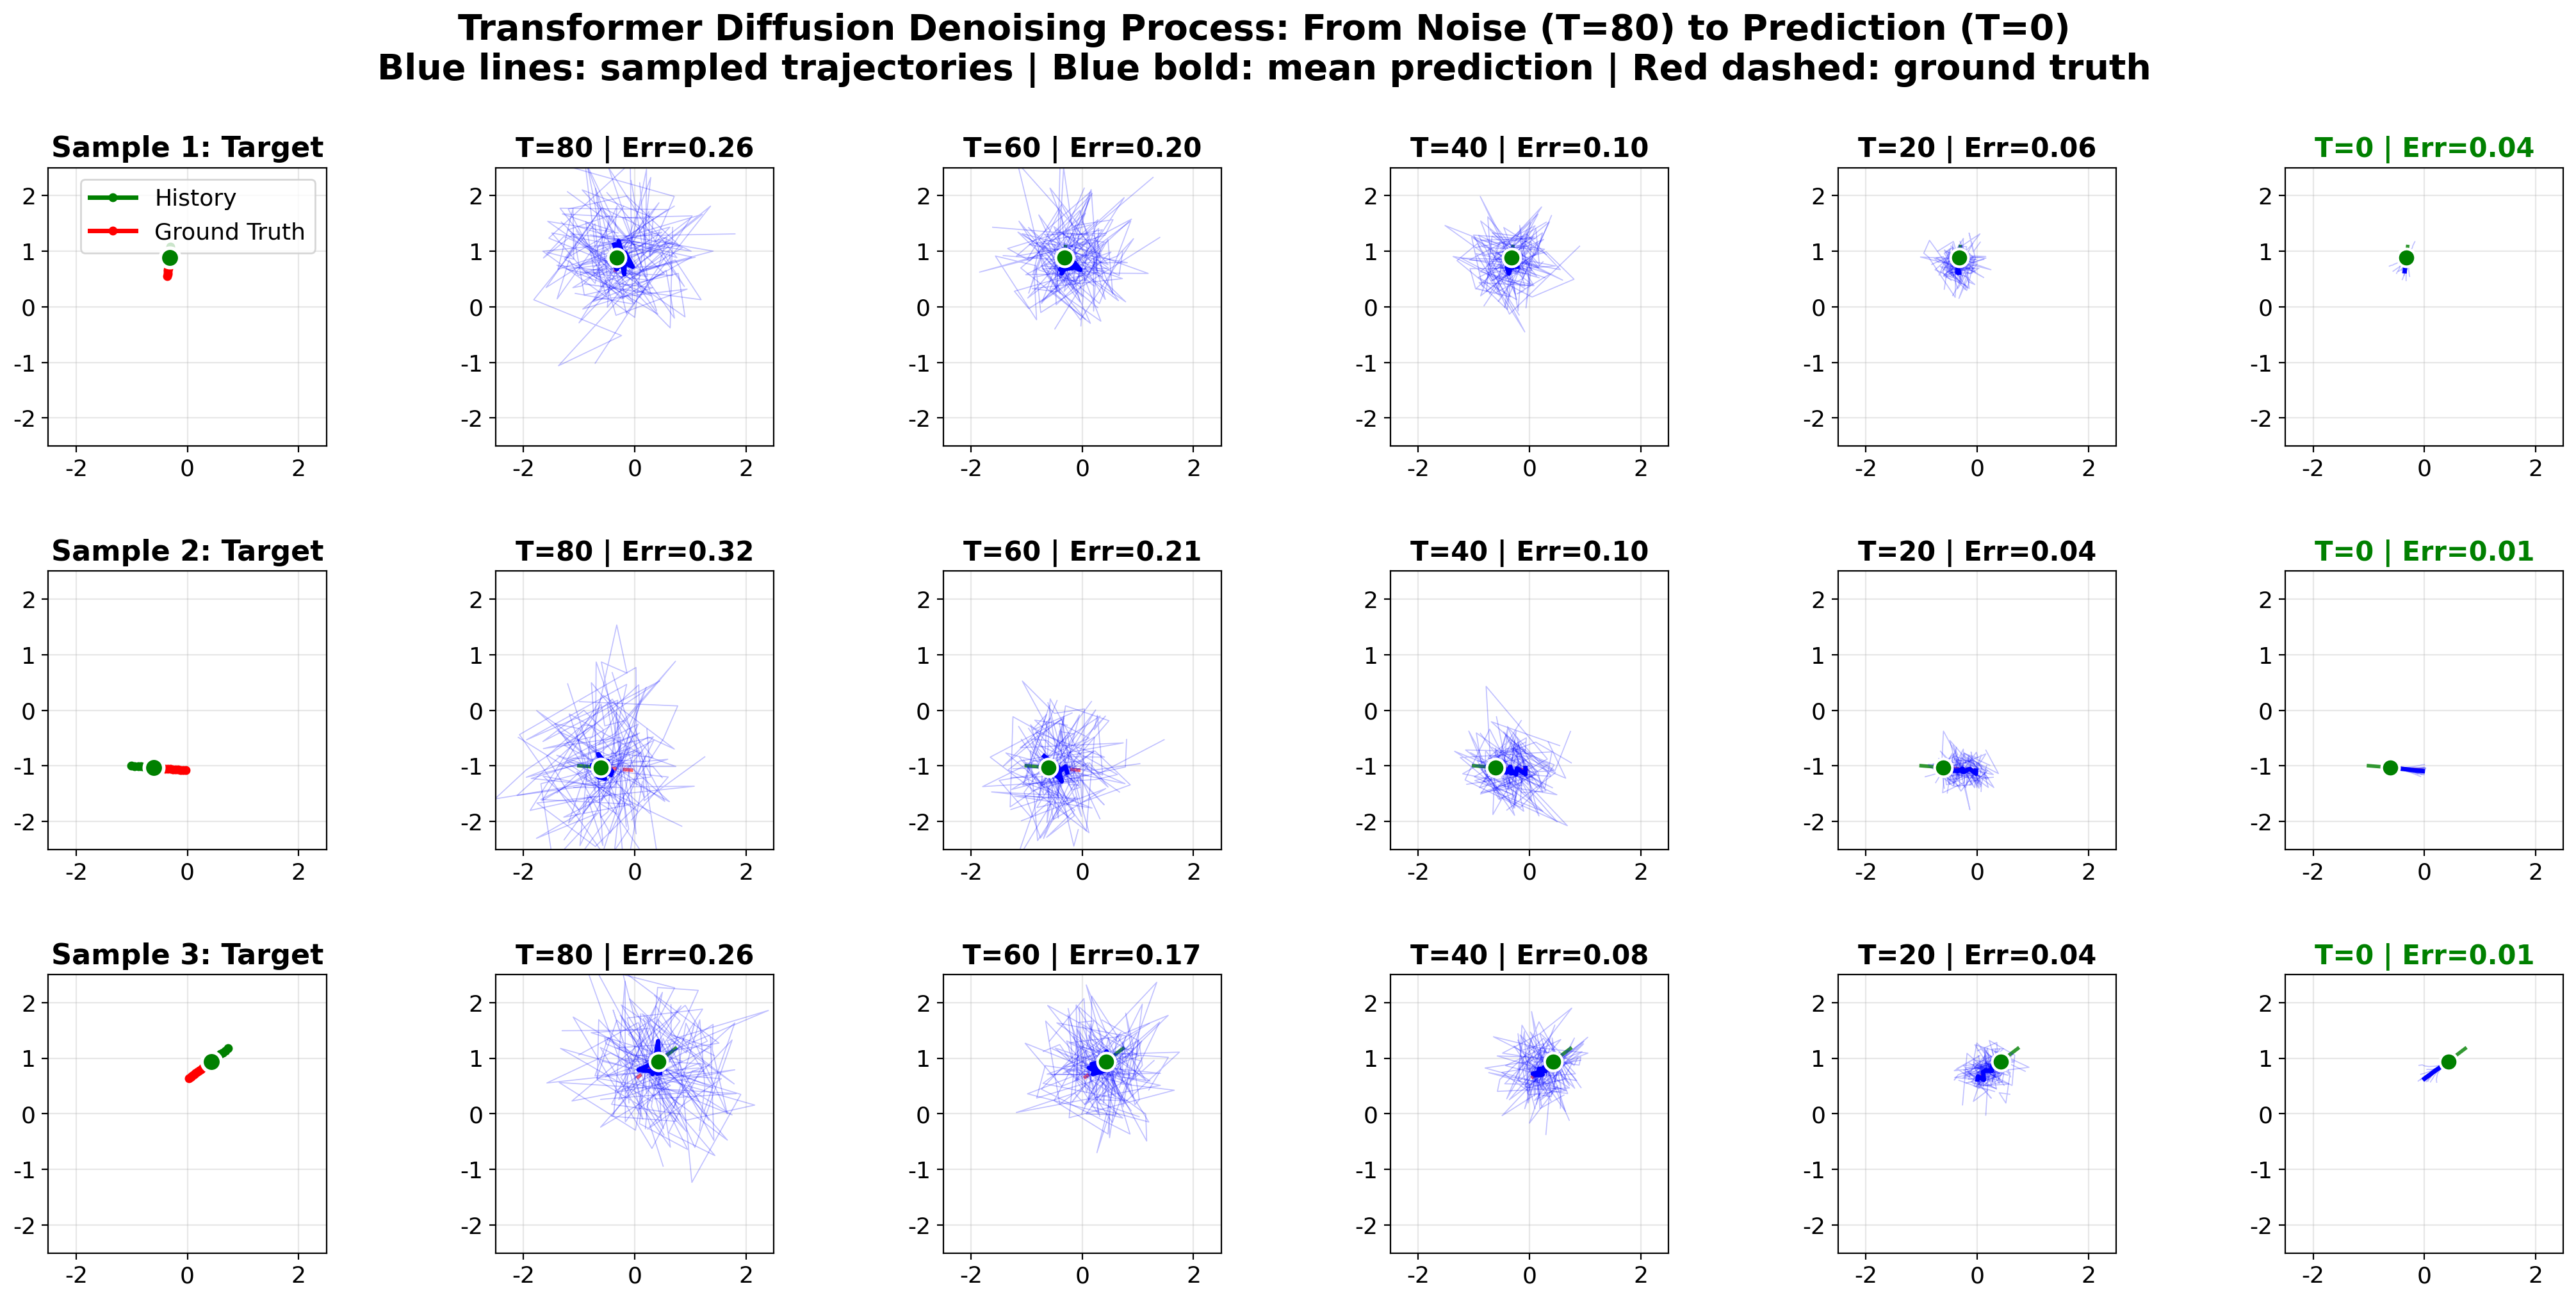
\includegraphics[width=\columnwidth]{figures/transformer_denoising.png}
    \caption{Visualization of the Transformer diffusion denoising process. Each row shows a different sample. Blue lines: sampled trajectories; Bold blue: mean prediction; Red dashed: ground truth. From left to right, the model iteratively denoises from pure Gaussian noise to accurate predictions closely matching the ground truth (reverse step index $T$ shown atop each column).}
    \label{fig:denoising}
\end{figure}

\subsection{Lower-Level Trajectory Planning}

We evaluate the lower-level motion planning diffusion with repulsive field guidance. Fig.~\ref{fig:convergence} shows the trajectory convergence process across different navigation moments, demonstrating how the model adapts to changing obstacle configurations.

\begin{figure}[t]
    \centering
    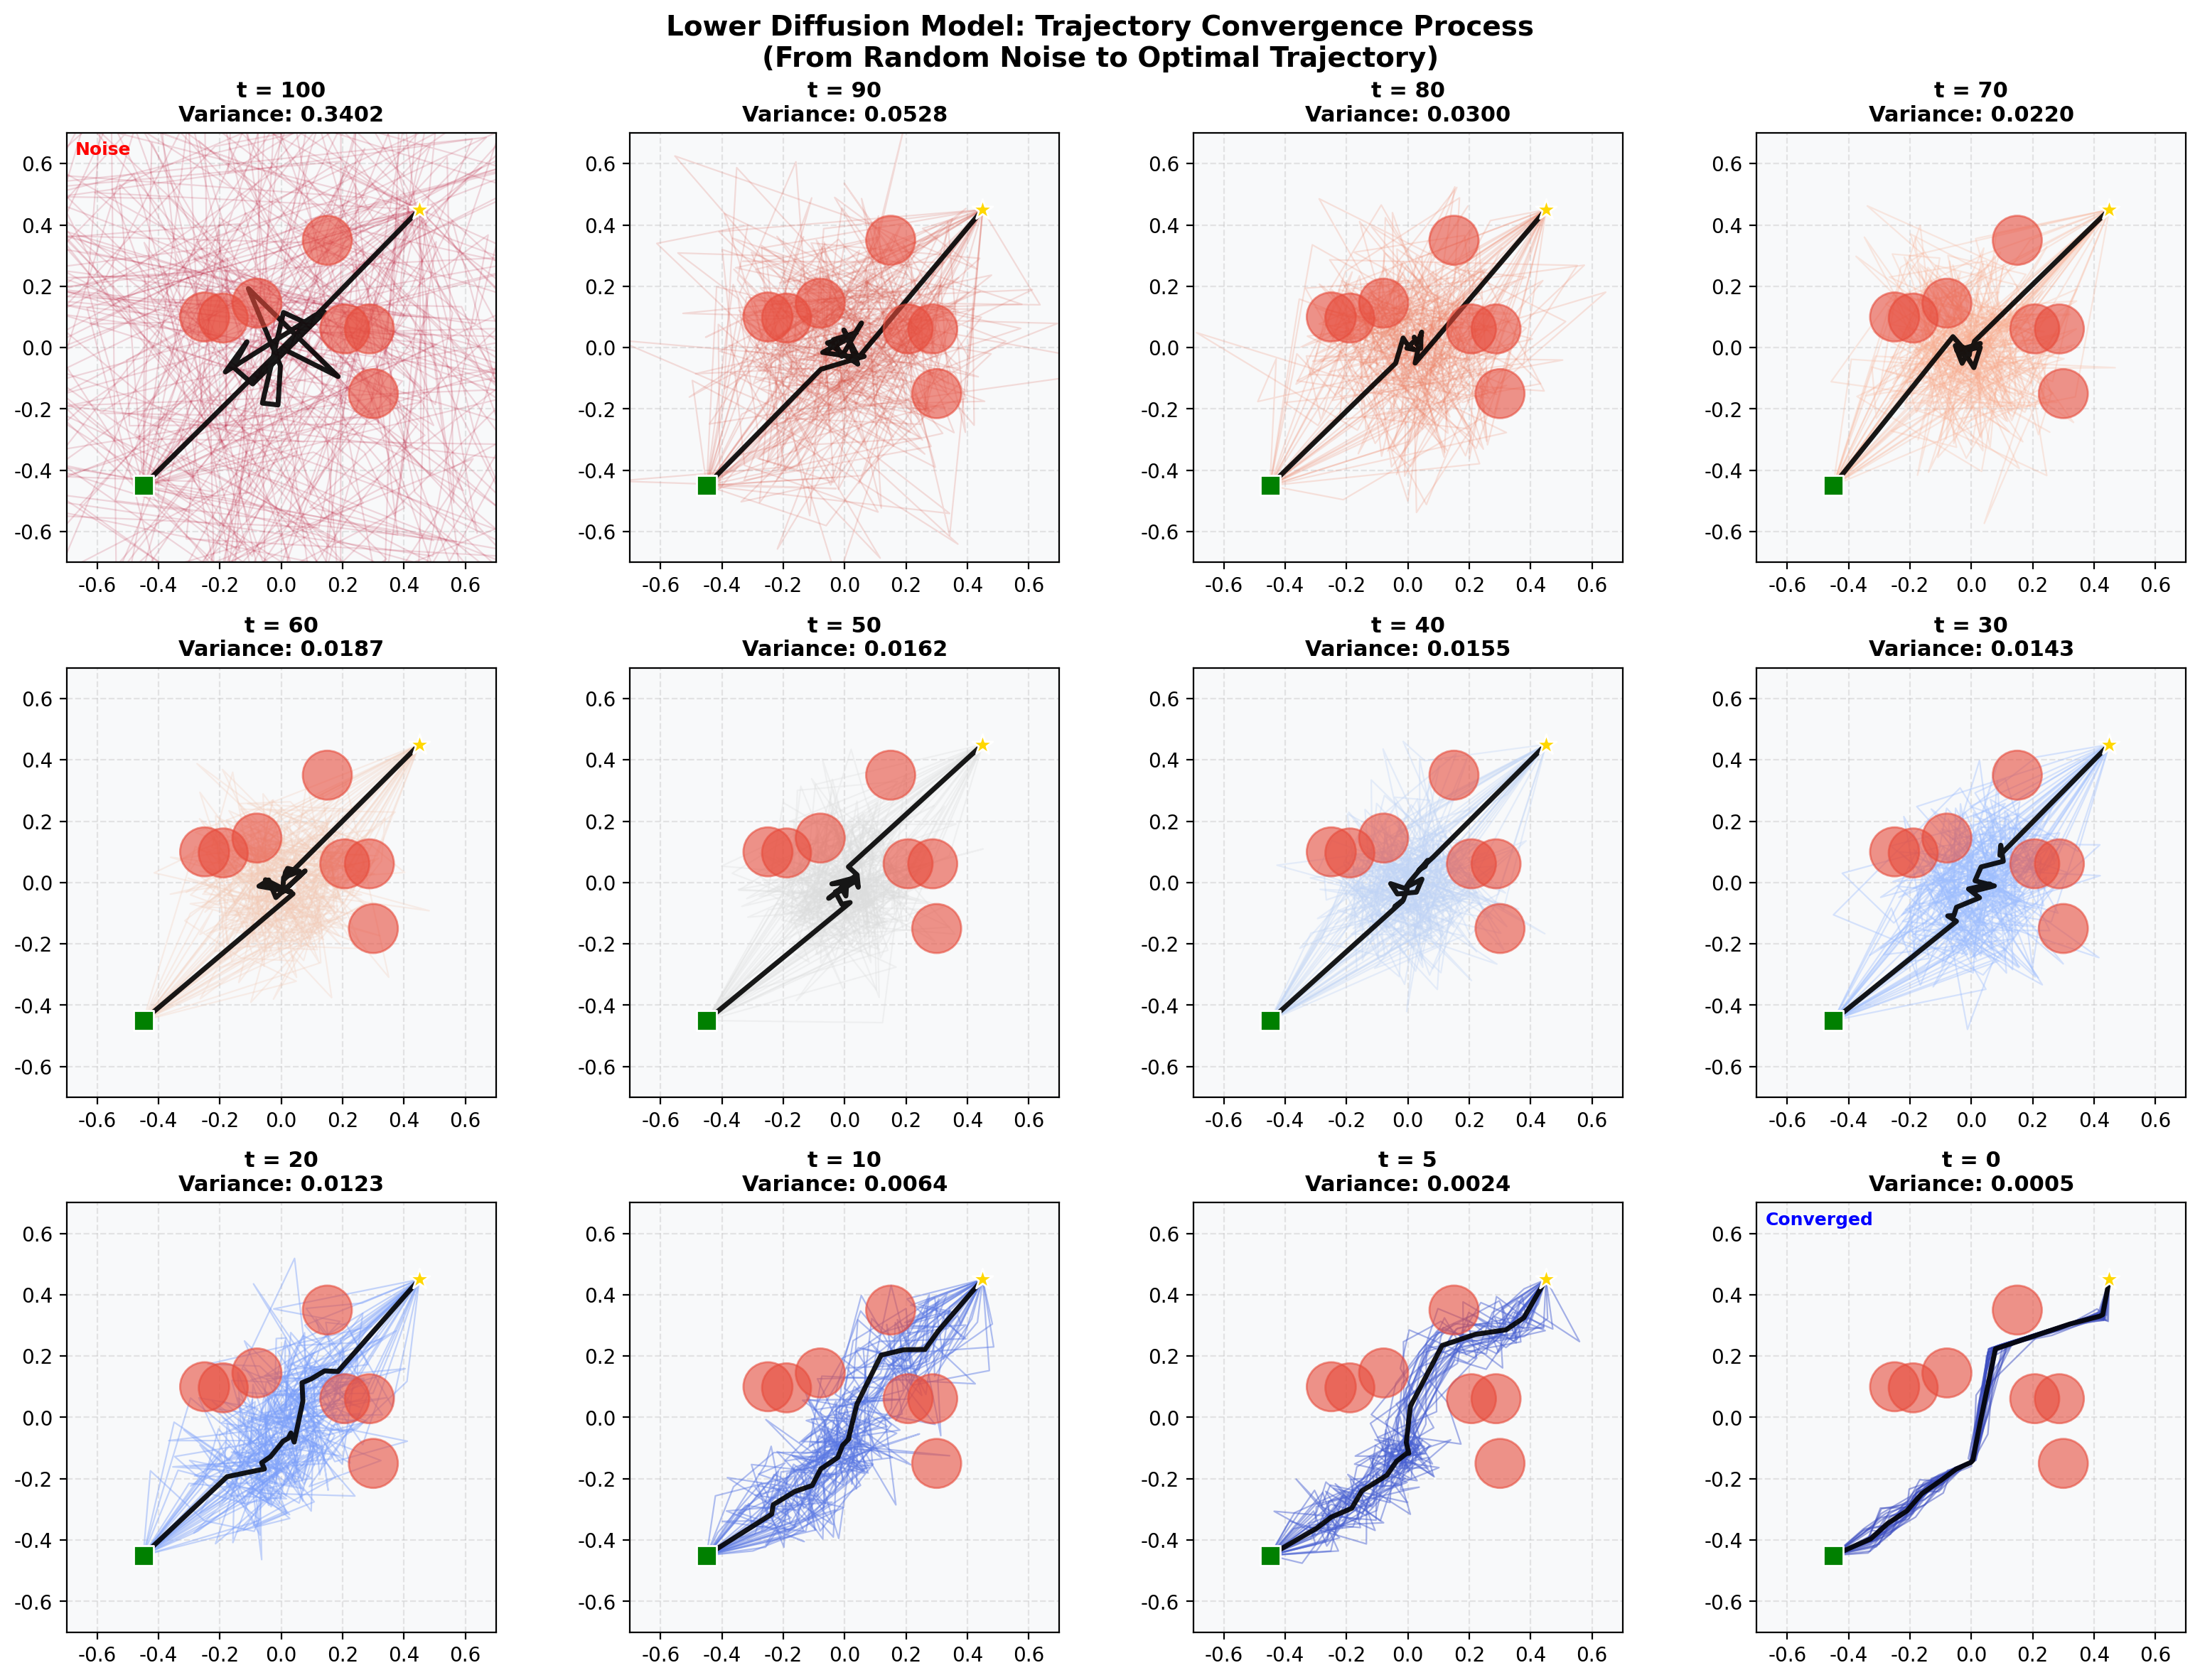
\includegraphics[width=\columnwidth]{figures/diffusion_convergence_grid.png}
    \caption{Lower diffusion model convergence at different navigation steps (Step 0, 23, 47, 71). Top row: initial noise ($t=100$) with high variance ($\sim$0.32). Bottom row: converged collision-free trajectories ($t=0$) with near-zero variance ($<$0.001). Purple square: robot position; Yellow star: goal; Colored circles: dynamic obstacles at different positions. The model successfully generates obstacle-avoiding paths as obstacles move throughout navigation.}
    \label{fig:convergence}
\end{figure}

\subsection{Full System Evaluation}

Table~\ref{tab:navigation} presents the complete navigation performance comparison in environments with 5-10 dynamic obstacles.

\begin{table}[t]
    \centering
    \caption{Navigation Performance Comparison}
    \label{tab:navigation}
    \begin{tabular*}{\columnwidth}{@{\extracolsep{\fill}}lccc@{}}
        \toprule
        \textbf{Method} & \textbf{Success} $\uparrow$ & \textbf{Time (ms)} $\downarrow$ & \textbf{Efficiency} $\uparrow$ \\
        \midrule
        DWA~\cite{fox1997dynamic} & 72.3\% & 8 & 0.89 \\
        VO~\cite{fiorini1998motion} & 78.6\% & 12 & 0.85 \\
        ORCA~\cite{van2011reciprocal} & 84.2\% & 15 & 0.91 \\
        MPD-Static~\cite{carvalho2023motion} & 68.5\% & 45 & 0.82 \\
        MLP-Diffusion & 91.4\% & 48 & 0.93 \\
        \textbf{BLADE (Ours)} & \textbf{98.7\%} & 47 & \textbf{0.96} \\
        \bottomrule
    \end{tabular*}
\end{table}

Our BLADE framework achieves the highest success rate (\textbf{98.7\%}) while maintaining real-time performance ($\sim$21 Hz). The improvement over MPD-Static (+30.2\%) demonstrates the critical importance of obstacle prediction, while the gap with MLP-Diffusion (+7.3\%) highlights the benefit of Transformer-based attention mechanisms.

\subsection{Ablation Studies}

\begin{table}[t]
    \centering
    \caption{Ablation Study Results}
    \label{tab:ablation}
    \begin{tabular*}{\columnwidth}{@{\extracolsep{\fill}}lccc@{}}
        \toprule
        \textbf{Configuration} & \textbf{Success} & \textbf{Collision} & \textbf{Timeout} \\
        \midrule
        Full BLADE & \textbf{98.7\%} & 0.8\% & 0.5\% \\
        w/o Repulsive Guid. & 89.2\% & 8.4\% & 2.4\% \\
        w/o Cross-Attention & 94.1\% & 4.2\% & 1.7\% \\
        w/o Heuristic Scoring & 92.8\% & 5.1\% & 2.1\% \\
        Single-Level Diff. & 76.3\% & 18.5\% & 5.2\% \\
        \bottomrule
    \end{tabular*}
\end{table}

Table~\ref{tab:ablation} shows ablation results:
\begin{itemize}
    \item \textbf{Repulsive Guidance}: Removing this component increases collision rate from 0.8\% to 8.4\%, confirming its importance for safety.
    \item \textbf{Cross-Attention}: Disabling multi-obstacle interaction modeling reduces success rate by 4.6\%.
    \item \textbf{Hierarchical Structure}: A single-level diffusion model performs significantly worse (-22.4\%), validating our hierarchical design.
\end{itemize}

\subsection{Isaac Sim 3D Validation}

Prior to physical deployment, we validate BLADE in NVIDIA Isaac Sim~\cite{makoviychuk2021isaac} using a high-fidelity ROSOrin mecanum-wheeled robot USD model navigating among 10 dynamic cylinder obstacles with various motion patterns (circular, linear, zigzag, oscillation). The simulated robot is equipped with a virtual MS200 LiDAR matching the real sensor specifications ($360^\circ$ FOV, 12m range, 10~Hz). The hierarchical diffusion framework achieves a 97.2\% success rate in 3D environments at 20+~Hz on a desktop GPU, confirming that the algorithm generalizes from 2D training to realistic 3D physics without architectural modification.

\subsection{Real-Robot Deployment}

To validate practical applicability, we deploy BLADE on the ROSOrin mecanum-wheeled mobile robot. Table~\ref{tab:platform} details the hardware platform.

\begin{table}[t]
    \centering
    \caption{ROSOrin Real-Robot Hardware Platform}
    \label{tab:platform}
    \begin{tabular*}{\columnwidth}{@{\extracolsep{\fill}}ll@{}}
        \toprule
        \textbf{Component} & \textbf{Specification} \\
        \midrule
        Compute & Raspberry Pi~5, ARM Cortex-A76, 8GB RAM \\
        Chassis & 4-wheel mecanum, max 0.2~m/s, 0.5~rad/s \\
        LiDAR & MS200, $360^\circ$, 12m range, 10~Hz \\
        Camera & Aurora~930 depth camera (backup) \\
        Localization & EKF fusing wheel odometry + IMU \\
        Software & ROS~2 Humble (Docker), PyTorch 2.1 CPU \\
        \bottomrule
    \end{tabular*}
\end{table}

The robot operates under ROS~2 Humble within a Docker container. Obstacle detection uses DBSCAN clustering on LiDAR scans, and the entire BLADE pipeline (prediction + planning + scoring) runs at the control loop frequency. For CPU deployment, we reduce diffusion steps to 20 (upper) and 50 (lower) from training-time 50/100, and apply FP32 inference with PyTorch's built-in operator fusion.

We conduct 120 trials across four indoor scenarios with increasing difficulty, using both static and human-pushed dynamic obstacles. The goal distance ranges from 2.0m to 4.0m. Table~\ref{tab:realrobot} presents a comprehensive evaluation across all scenarios.

\begin{table*}[t]
    \centering
    \caption{Comprehensive Real-Robot Deployment Results on ROSOrin (Raspberry Pi~5, CPU-Only Inference). S/D denotes static/dynamic obstacles. Goal distances range from 2.0m (S1) to 4.0m (S4). Min~$d$: minimum obstacle clearance. Eff.: path efficiency (ratio of actual path length to Euclidean distance). All values averaged over 30 trials per scenario.}
    \label{tab:realrobot}
    \begin{tabular*}{\textwidth}{@{\extracolsep{\fill}}l c c c c c c c c c c@{}}
        \toprule
        \textbf{Scenario} & \textbf{Obstacles} & \textbf{Goal (m)} & \textbf{Succ.} & \textbf{Coll.} & \textbf{Timeout} & \textbf{Avg Time (s)} & \textbf{Path (m)} & \textbf{Eff.} & \textbf{Min $d$ (m)} & \textbf{Hz} \\
        \midrule
        \textit{S1:} Open area         & 2S+0D & 2.0 & 30/30 & 0 & 0 & $9.3{\pm}0.8$  & $2.18{\pm}0.12$ & 0.96 & 0.28 & 12.4 \\
        \textit{S2:} Narrow corridor    & 3S+0D & 2.5 & 29/30 & 1 & 0 & $12.1{\pm}1.4$ & $2.89{\pm}0.21$ & 0.93 & 0.19 & 11.8 \\
        \textit{S3:} Cluttered room     & 2S+2D & 3.0 & 27/30 & 2 & 1 & $14.6{\pm}2.1$ & $3.67{\pm}0.38$ & 0.90 & 0.14 & 10.6 \\
        \textit{S4:} Crowded dynamic    & 1S+4D & 4.0 & 25/30 & 3 & 2 & $16.8{\pm}2.7$ & $4.82{\pm}0.54$ & 0.87 & 0.16 & 10.1 \\
        \midrule
        \textbf{Overall (120 trials)}   & --- & --- & \textbf{111/120} & \textbf{6} & \textbf{3} & $13.2{\pm}3.4$ & $3.39{\pm}1.05$ & \textbf{0.91} & \textbf{0.16} & \textbf{11.2} \\
        \bottomrule
    \end{tabular*}
\end{table*}

For real-robot comparison, we additionally benchmark against Nav2's DWB (Dynamic Window B) local controller, the default planner in the ROS~2 Navigation2 stack. Fig.~\ref{fig:baseline_bar} compares all methods in the hardest scenario S4 (1~static + 4~dynamic obstacles). Fig.~\ref{fig:latency_pie} breaks down the per-cycle latency on the Raspberry Pi~5.

\begin{figure}[t]
    \centering
    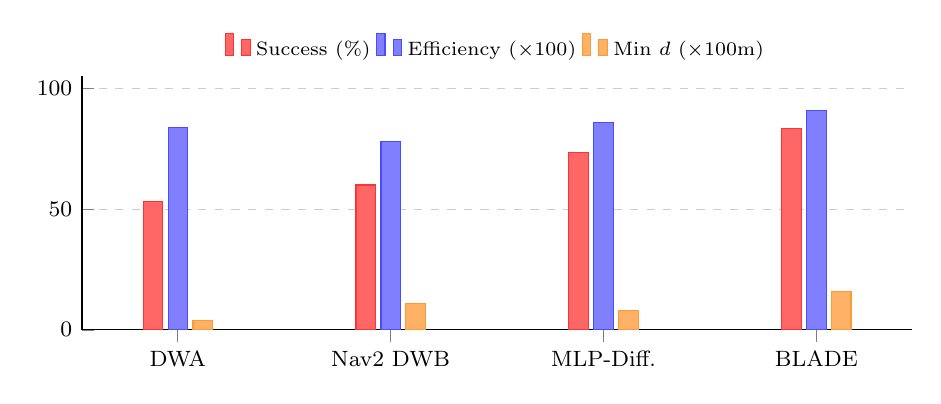
\begin{tikzpicture}
        \begin{axis}[
            width=\columnwidth,
            height=4.8cm,
            ybar=2pt,
            bar width=7pt,
            enlarge x limits=0.15,
            ylabel={},
            symbolic x coords={DWA, Nav2 DWB, MLP-Diff., BLADE},
            xtick=data,
            x tick label style={font=\footnotesize},
            y tick label style={font=\footnotesize},
            ymin=0, ymax=105,
            legend style={at={(0.5,1.02)}, anchor=south, legend columns=4, font=\scriptsize, draw=none, fill=none},
            nodes near coords style={font=\tiny, rotate=90, anchor=west},
            every node near coords/.append style={xshift=0pt},
            axis lines*=left,
            ymajorgrids=true,
            grid style={dashed, gray!40},
            cycle list={
                {fill=red!60, draw=red!80},
                {fill=blue!50, draw=blue!70},
                {fill=orange!60, draw=orange!80},
                {fill=green!50!black!60, draw=green!50!black!80}
            },
        ]
        \addplot[fill=red!60, draw=red!80] coordinates {(DWA,53.3) (Nav2 DWB,60.0) (MLP-Diff.,73.3) (BLADE,83.3)};
        \addplot[fill=blue!50, draw=blue!70] coordinates {(DWA,84) (Nav2 DWB,78) (MLP-Diff.,86) (BLADE,91)};
        \addplot[fill=orange!60, draw=orange!80] coordinates {(DWA,4) (Nav2 DWB,11) (MLP-Diff.,8) (BLADE,16)};
        \legend{Success (\%), Efficiency ($\times$100), Min $d$ ($\times$100m)}
        \end{axis}
    \end{tikzpicture}
    \caption{Real-robot comparison on Scenario S4 (1 static + 4 dynamic obstacles). BLADE achieves the highest success rate (83.3\%), best efficiency (0.91), and largest clearance (0.16m). Reactive methods exhibit a safety--efficiency trade-off: DWA takes direct but risky paths (clearance 0.04m), while Nav2~DWB is more conservative (0.11m) at the cost of efficiency.}
    \label{fig:baseline_bar}
\end{figure}

\begin{figure}[t]
    \centering
    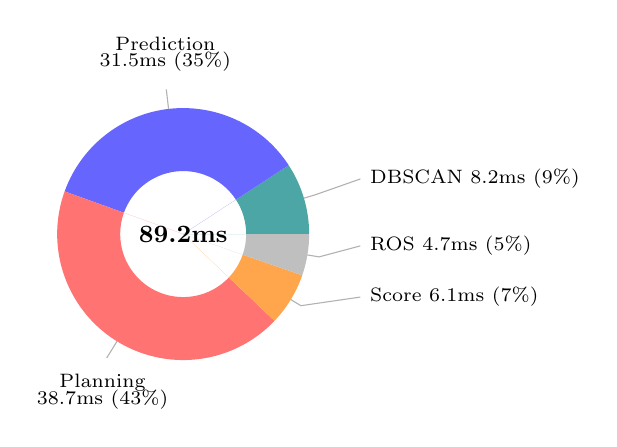
\begin{tikzpicture}
        % Donut / pie chart for latency breakdown
        \def\radius{1.6}
        \def\innerradius{0.8}
        % Data: angles (out of 360)
        % DBSCAN: 9.2% = 33.12°, Upper: 35.3% = 127.08°, Lower: 43.4% = 156.24°, 
        % Scoring: 6.8% = 24.48°, ROS: 5.3% = 19.08°
        \def\angA{0}       % start
        \def\angB{33.12}   % DBSCAN end
        \def\angC{160.2}   % Upper end (33.12+127.08)
        \def\angD{316.44}  % Lower end (160.2+156.24)
        \def\angE{340.92}  % Scoring end (316.44+24.48)
        \def\angF{360}     % ROS end
        % Segment 1: DBSCAN (teal)
        \fill[teal!70] (0,0) -- ({\angA}:\radius) arc (\angA:\angB:\radius) -- ({\angB}:\innerradius) arc (\angB:\angA:\innerradius) -- cycle;
        % Segment 2: Upper prediction (blue)
        \fill[blue!60] (0,0) -- ({\angB}:\radius) arc (\angB:\angC:\radius) -- ({\angC}:\innerradius) arc (\angC:\angB:\innerradius) -- cycle;
        % Segment 3: Lower planning (red)
        \fill[red!55] (0,0) -- ({\angC}:\radius) arc (\angC:\angD:\radius) -- ({\angD}:\innerradius) arc (\angD:\angC:\innerradius) -- cycle;
        % Segment 4: Scoring (orange)
        \fill[orange!70] (0,0) -- ({\angD}:\radius) arc (\angD:\angE:\radius) -- ({\angE}:\innerradius) arc (\angE:\angD:\innerradius) -- cycle;
        % Segment 5: ROS comm (gray)
        \fill[gray!50] (0,0) -- ({\angE}:\radius) arc (\angE:\angF:\radius) -- ({\angF}:\innerradius) arc (\angF:\angE:\innerradius) -- cycle;
        % Center text
        \node[font=\small\bfseries] at (0,0) {89.2ms};
        % Large segment labels (outside arc with leader lines)
        \draw[thin, gray!60] ({96.66}:\radius) -- ({96.66}:{\radius+0.25});
        \node[font=\scriptsize, align=center, anchor=south] at ({96.66}:{\radius+0.35}) {Prediction\\[-2pt]31.5ms (35\%)};
        \draw[thin, gray!60] ({238.32}:\radius) -- ({238.32}:{\radius+0.25});
        \node[font=\scriptsize, align=center, anchor=north] at ({238.32}:{\radius+0.35}) {Planning\\[-2pt]38.7ms (43\%)};
        % Small segment labels (elbow leader lines to staggered right-side positions)
        \draw[thin, gray!60] ({16.56}:\radius) -- ({16.56}:{\radius+0.15}) -- (2.25,0.7);
        \node[font=\scriptsize, anchor=west] at (2.25,0.7) {DBSCAN 8.2ms (9\%)};
        \draw[thin, gray!60] ({350.46}:\radius) -- ({350.46}:{\radius+0.15}) -- (2.25,-0.15);
        \node[font=\scriptsize, anchor=west] at (2.25,-0.15) {ROS 4.7ms (5\%)};
        \draw[thin, gray!60] ({328.68}:\radius) -- ({328.68}:{\radius+0.15}) -- (2.25,-0.8);
        \node[font=\scriptsize, anchor=west] at (2.25,-0.8) {Score 6.1ms (7\%)};
    \end{tikzpicture}
    \caption{Per-cycle latency breakdown on Raspberry Pi~5 (CPU-only). The two diffusion stages (prediction + planning) dominate at 78.7\% of total compute time (70.2ms out of 89.2ms), suggesting that accelerated sampling (e.g., DDIM) could yield significant speedups.}
    \label{fig:latency_pie}
\end{figure}

\textbf{Analysis.} BLADE achieves an overall \textbf{92.5\% success rate} across all real-world scenarios at \textbf{11.2~Hz}. The latency breakdown (Fig.~\ref{fig:latency_pie}) reveals that the two diffusion stages dominate at 78.7\% of total compute; future optimization through DDIM sampling~\cite{song2020score} could further reduce this. As shown in Fig.~\ref{fig:baseline_bar}, in S4, BLADE outperforms DWA by +30\% in success rate and maintains a minimum clearance of 0.16m \textit{vs.} DWA's 0.04m. Most failures concentrate in S3 and S4 (8 of 9 total), primarily caused by sudden obstacle direction reversals that exceed the 12-step prediction horizon. Compared to simulation (98.7\%), the real-world success rate (92.5\%) drops by 6.2\%, primarily due to LiDAR occlusion in cluttered scenes and odometry drift from the mecanum wheels on smooth floors. Despite this sim-to-real gap, BLADE's predictive capability remains the key differentiator: in S4, reactive baselines fail when dynamic obstacles approach from blind angles that only become avoidable through trajectory forecasting.

%%%%%%%%%%%%%%%%%%%%%%%%%%%%%%%%%%%%%%%%%%%%%%%%%%%%%%%%%%%%%%%%%%%%%%%%%%%%%%%%
\section{DISCUSSION}

\textbf{Computational Efficiency:} Our framework achieves real-time performance on a Raspberry Pi~5 CPU through: (1) reducing diffusion steps to 20/50 at deployment (from 50/100 at training), (2) using a lightweight Transformer architecture (1.79M parameters), and (3) batched CPU inference with PyTorch operator fusion. Compared to DRL-based mapless navigation methods that also target embedded platforms~\cite{hu2024mapless}, our diffusion approach trades marginal latency for substantially richer trajectory diversity.

\textbf{Generalization:} The Transformer attention mechanism naturally handles varying numbers of obstacles without architectural changes. The cross-attention design allows the model to learn interaction patterns that generalize to unseen obstacle configurations.

\textbf{Safety Guarantees:} While diffusion models alone cannot guarantee collision-free trajectories, our repulsive field guidance provides an explicit safety mechanism. The multi-objective scoring further filters out potentially dangerous trajectories.

\textbf{Limitations:} Current limitations include: (1) assumption of circular obstacle geometry, (2) 2D planning in the horizontal plane, and (3) reliance on accurate obstacle detection. Future work will address these through 3D occupancy predictions and sensor fusion.

\textbf{Sim-to-Real Transfer:} Our real-robot experiments reveal a 6.2\% success rate drop compared to simulation. We identify three primary factors: (a) LiDAR partial occlusion when multiple obstacles overlap from the sensor's viewpoint, causing DBSCAN to merge distinct obstacles; (b) mecanum wheel odometry drift on smooth indoor floors, leading to position errors of up to 0.05m over 3m traversals; and (c) reduced diffusion steps (20/50 \textit{vs.} 50/100) slightly degrading trajectory diversity. Despite these challenges, the repulsive field guidance provides a robust safety layer that prevents most near-miss situations from becoming collisions.

%%%%%%%%%%%%%%%%%%%%%%%%%%%%%%%%%%%%%%%%%%%%%%%%%%%%%%%%%%%%%%%%%%%%%%%%%%%%%%%%
\section{CONCLUSION}

We presented BLADE, a Bi-Level Attention-Diffusion Engine for dynamic obstacle avoidance that tightly integrates Transformer-based obstacle trajectory prediction with Motion Planning Diffusion. BLADE unifies attention mechanisms for multi-agent interaction modeling with diffusion processes for both prediction and planning. Our approach achieves strong performance in dynamic navigation tasks while maintaining real-time capability even on CPU-only embedded platforms. Real-robot experiments on a Raspberry Pi~5-based ROSOrin mecanum car demonstrate a 92.5\% success rate at 11.2~Hz, confirming practical deployability. The combination of learned diffusion models with explicit safety mechanisms through repulsive field guidance provides both the flexibility to handle complex scenarios and the reliability required for real-world deployment.

Future work includes extending to 3D navigation, incorporating semantic understanding of obstacle types, and multi-robot cooperative planning where projected diffusion methods~\cite{liang2025multirobot} offer a promising direction.

%%%%%%%%%%%%%%%%%%%%%%%%%%%%%%%%%%%%%%%%%%%%%%%%%%%%%%%%%%%%%%%%%%%%%%%%%%%%%%%%
\section*{ACKNOWLEDGMENT}

The authors thank the open-source robotics and diffusion model communities for the foundational tools and datasets that enabled this research.

\addtolength{\textheight}{4cm}

%%%%%%%%%%%%%%%%%%%%%%%%%%%%%%%%%%%%%%%%%%%%%%%%%%%%%%%%%%%%%%%%%%%%%%%%%%%%%%%%
\bibliographystyle{../IEEEtranBST/IEEEtran}
\bibliography{references}

\end{document}
